\documentclass{article}
\usepackage[utf8x]{inputenc}
\usepackage{ucs}
\usepackage{amsmath} 
\usepackage{amsfonts}
\usepackage{marvosym}
\usepackage{wasysym}
\usepackage{upgreek}
\usepackage[english,russian]{babel}
\usepackage{graphicx}
\usepackage{float}
\usepackage{textcomp}
\usepackage{hyperref}
\usepackage{geometry}
  \geometry{left=2cm}
  \geometry{right=1.5cm}
  \geometry{top=1cm}
  \geometry{bottom=2cm}
\usepackage{tikz}
\usepackage{ccaption}
\usepackage{multicol}

\hypersetup{
   colorlinks=true,
   citecolor=blue,
   linkcolor=black,
   urlcolor=blue
}

\usepackage{listings}
%\setlength{\columnsep}{1.5cm}
%\setlength{\columnseprule}{0.2pt}

\usepackage[absolute]{textpos}

\usepackage{colortbl,graphicx,tikz}
\definecolor{X}{rgb}{.5,.5,.5}


\begin{document}
\pagenumbering{gobble}
\lstset{
  language=C,                % choose the language of the code
  basicstyle=\linespread{1.1}\ttfamily,
  columns=fixed,
  fontadjust=true,
  basewidth=0.5em,
  keywordstyle=\color{blue}\bfseries,
  commentstyle=\color{gray},
  stringstyle=\ttfamily\color{orange!50!black},
  showstringspaces=false,
  numbersep=5pt,
  numberstyle=\tiny\color{black},
  numberfirstline=true,
  stepnumber=1,                   % the step between two line-numbers.        
  numbersep=10pt,                  % how far the line-numbers are from the code
  backgroundcolor=\color{white},  % choose the background color. You must add \usepackage{color}
  showstringspaces=false,         % underline spaces within strings
  captionpos=b,                   % sets the caption-position to bottom
  breaklines=true,                % sets automatic line breaking
  breakatwhitespace=true,         % sets if automatic breaks should only happen at whitespace
  xleftmargin=.2in,
  extendedchars=\true,
  keepspaces = true,
}
\lstset{literate=%
   *{0}{{{\color{red!20!violet}0}}}1
    {1}{{{\color{red!20!violet}1}}}1
    {2}{{{\color{red!20!violet}2}}}1
    {3}{{{\color{red!20!violet}3}}}1
    {4}{{{\color{red!20!violet}4}}}1
    {5}{{{\color{red!20!violet}5}}}1
    {6}{{{\color{red!20!violet}6}}}1
    {7}{{{\color{red!20!violet}7}}}1
    {8}{{{\color{red!20!violet}8}}}1
    {9}{{{\color{red!20!violet}9}}}1
}
\newpage

\title{Семинар \#8: Память. Классные задания.\vspace{-5ex}}\date{}\maketitle
\section*{Часть 1: Системы счисления}
Мы привыкли пользоваться десятичной системой счисления и не задумываемся, что под числом в десятичной записи подразумевается следующее:
$$
123.45_{10} = 1 \cdot 10^2 + 2 \cdot 10^1 + 3 \cdot 10^0 + 4 \cdot 10^{-1} + 5 \cdot 10^{-2}
$$
Конечно, в числе 10 нет ничего сильно особенного с математической точки зрения. Оно было выбрано исторически, скорей всего по той причине, что у человека 10 пальцев. Компьютеры же работают с двоичными числами, потому что оказалось что процессоры на основе двоичной логики сделать проще. В двоичной системе счисления есть всего 2 цифры: \texttt{0} и \texttt{1}. Под записью числа в двоичной системе подразумевается примерно то же самое, что и в десятичной:
$$
101.01_2 = 1 \cdot 2^2 + 0 \cdot 2^1 + 1 \cdot 2^0 + 0 \cdot 2^{-1} + 1 \cdot 2^{-2} = 5.25_{10}
$$
При работе с компьютером на низком уровне имеет смысл использовать двоичную систему за место десятичной.  Но человеку очень сложно воспринимать числа в двоичной записи, так как они получаются слишком длинными. Поэтому популярность приобрели восьмеричная и шестнадцатиричная системы счисления. В шестнадцатиричной системе счисления есть 16 цифр: \texttt{0, 1, 2, 3, 4, 5, 6, 7, 8, 9, a, b, c, d, e, f}.
$$
1a.8_{16} = 1 \cdot 16^1 + 10 \cdot 16^0 + 8 \cdot 16^{-1} = 26.5_{10}
$$
\subsubsection*{Задача. Переводите следующие числа в десятичную систему:}
\begin{multicols}{3}
\begin{itemize}
\item[--] $11011_2$
\item[--] $1.1_2$
\item[--] $2b_{16}$
\item[--] $a.c_{16}$
\item[--] $40_{8}$
\item[--] $10_{123}$
\end{itemize}
\end{multicols}

\subsection*{Шестнадцатиричная и восьмеричная системы в языке \texttt{C}:}
Язык \texttt{C} поддерживает шестнадцатиричные и восьмеричные числа. Чтобы получить восьмеричное число нужно написать \texttt{0} перед числом. Чтобы получить шестнадцатиричное число нужно написать \texttt{0x} перед числом.
\begin{lstlisting}
#include <stdio.h>
int main() 
{
    int a = 123;    // Десятичная система
    int b = 0123;   // Восьмеричная система
    int c = 0x123;  // Шестнадцатиричная система
    printf("%i %i %i\n", a, b, c);
}
\end{lstlisting}
Также, можно печатать и считывать числа в этих системах счисления с помощью спецификаторов \texttt{\%o} (для восьмеричной системы -- \textbf{o}ctal) и \texttt{\%x} (для шестнадцатеричной -- he\textbf{x}adecimal). Спецификатор \texttt{\%d} можно использовать для десятичной системы -- \textbf{d}ecimal. Пример программы, которая считывает число в шестнадцатеричной системе и печатает в десятичной:
\begin{lstlisting}
#include <stdio.h>
int main() 
{
    int a;
    scanf("%x", &a);
    printf("%d\n", a);
}
\end{lstlisting}
\newpage
\section*{Часть 2: Переменные в памяти. Little и Big Endian}
Положение любой переменной в памяти характеризуется двумя числами: её адресом(номером первого байта этой переменной) и её размером. Рассмотрим ситуацию, когда были созданы 3 переменные типов \texttt{int} (размер 4 байта), \texttt{char} (размер 1 байт) и \texttt{float} (размер 4 байта).
На рисунке представлено схематическое расположение этих переменных в памяти (одному квадратику соответствует 1 байт):

\begin{center}
\includegraphics[scale=1]{../images/memory/memory_2_different_types.png}
\end{center}
Какие выводы можно сделать из этого изображения:
\begin{itemize}
\item Значение одного байта памяти удобно представлять двузначным шестнадцатиричным числом.
\item Каждая переменная заняла столько байт, чему равен её размер.
\item Переменные в памяти могут хранится не в том порядке, в котором вы их объявляете.
\item Переменные в памяти хранятся не обязательно вплотную друг к другу.
\item Байты переменных \texttt{a} и \texttt{b} хранятся в обратном порядке. Такой порядок байт называется \texttt{Little Endian}.  Обратите внимание, что обращается только порядок байт, а не бит. Большинство компьютеров применяют именно такой порядок байт. Но в некоторых системах может использоваться обычный порядок байт -- \texttt{Big Endian}. Обратный порядок байт применяется не только к типу \texttt{int}, но и ко всем базовым типам.
\item Переменная \texttt{b} хранит ASCII-код символа \texttt{A}. Он который равен $65 = 41_{16}$.
\end{itemize}

\section*{Часть 3: Указатели разных типов}
Как вы могли заметить тип указателя зависит от типа элемента на который он указывает. Но все указатели, независимо от типа, по сути хранят одно и то же (адрес первого байта переменной). Чем же они различаются друг от друга? Разница проявляется как раз при их разыменовывании . Например, при разыменовывании указатель \texttt{int*} берёт 4 байта и воспринимает их как переменную типа \texttt{int}, а указатель \texttt{char*} берёт 1 байт и воспринимает его как переменную типа \texttt{char}.\\

Рассмотрим следующий пример. На переменную \texttt{a} указывают две переменные разных типов: \texttt{int*} и \texttt{char*}. Оба указателя хранят одно и то же значение, но работают по разному при разыменовании.

\begin{multicols}{2}
\begin{lstlisting}
#include <stdio.h>
int main() {
    int a = 0x12345678;
    int* p = &a;
    char* q = &a;
    
    printf("%p %p\n", p, q);
    printf("%x\n", *p);
    printf("%x\n", *q);
}
\end{lstlisting}
\vfill
\columnbreak
\hfill \break
\begin{center}
\includegraphics[scale=0.65]{../images/memory/memory_int_char_pointer.png}
\end{center}
\hfill \break
\end{multicols}

\subsection*{Преобразование типов указателя}
В предыдущем примере есть такая строка \texttt{char* p = \&a;} Необычность этой строки в том, что слева и справа от знака \texttt{=} находятся объекты разных типов. Слева -- \texttt{char*}, а справа -- \texttt{int*}. В этот момент происходит неявное преобразование типов один тип указателя преобразуется в другой. Это всё похоже на преобразование типов обычных переменных.
\begin{lstlisting}
int a = 4.1;         // Неявное преобразование из double в int
int b = (int)4.1;    // Явное преобразование из double в int

char* p = &a;        // Неявное преобразование из int* в char*  ( не работает в C++ )
char* p = (char*)&a; // Явное преобразование  из int* в char*
\end{lstlisting}
Надо отметить, что язык \texttt{C++} строже относится к соблюдению типов, чем язык \texttt{C}, и не позволит вам неявно преобразовать указатель одного типа в указатель другого типа.

\subsubsection*{Задача: Что напечатает следующая программа и почему она это напечатает?}
\begin{lstlisting} 
#include <stdio.h>
int main() {
    int a = 7627075;
    char* p = (char*)&a;
    printf("%s\n", p);
}
\end{lstlisting}
\subsection*{Указатель \texttt{void*}}
Помимо обычных указателей в языке есть специальный указатель \texttt{void*}. Этот указатель не ассоциирован не с каким типом, а просто хранит некоторый адрес. При попытке его разыменования произойдёт ошибка.
\subsubsection*{Задача:}
\begin{lstlisting} 
int a = 123;
void* p = (void*)&a;
\end{lstlisting}
Увеличьте переменную \texttt{a} в 2 раза и напечатайте её используя только указатель \texttt{p}.


\newpage

\section*{Часть 4: Просмотр байт}
\subsection*{Просмотр байт переменной}
Просмотреть, что содержится в байтах какого-либо объекта можно с помощью указателя на \texttt{unsigned char}.

\begin{lstlisting} 
#include <stdio.h>
int main() 
{
    int a = 0x11223344;
    
    unsigned char* p = (unsigned char*)&a;
    for (size_t i = 0; i < sizeof(a); ++i)
        printf("%x ", *(p + i));
    printf("\n");
}
\end{lstlisting}

\subsubsection*{Задача:}

\begin{itemize}
\item Напечатайте байты объекта \texttt{a} типа \texttt{double}.
\begin{lstlisting} 
double a = 123.456;
\end{lstlisting}

\item Напечатайте байты объекта \texttt{b} типа \texttt{int}.
\begin{lstlisting} 
int b = -1;
\end{lstlisting}

\item Напечатайте байты объекта \texttt{c} типа \texttt{struct cat}.
\begin{lstlisting} 
struct cat
{
    char first;
    int second;
};

int main()
{
    struct cat c = {0x50, 0x12345678}
}

\end{lstlisting}


\end{itemize}


\subsection*{Просмотр байтов файла с помощью программы \texttt{xxd}}
\textbf{\texttt{xxd}} - это простая программа, которая выводит на экран всё содержимое файла побайтово. Если, например, запустить программму следующим образом:
\texttt{xxd a.out}, то она выведет на экран всё содержимое этого исполняемого файла. Часто используемые опции командной строки: \texttt{-h} (сокращение от help) и \texttt{-v} (сокращение от version).
\begin{itemize}
\item Запустите \texttt{xxd} с аргументом -- именем файла \texttt{hello.txt}. Этот файл содержит лишь строку \texttt{Hello}.\\ 
\texttt{xxd} покажет вам содержимое этого файла в шестнадцатеричном виде и в виде \texttt{ASCII}.
\item Запустите \texttt{xxd} с опцией \texttt{-h}.
\item Запустите \texttt{xxd} с нужной опцией, чтобы вывод файла \texttt{hello.txt} был представлен в двоичном виде.
\item \textbf{*} Если файл большой, то весь вывод \texttt{xxd} не поместится на экран. Перенаправить вывод в нужный файл можно следующим образом:
\texttt{xxd a.out > temp.txt}. После этого в файле \texttt{temp.txt} будет хранится всё, что было бы напечатано на экран.
\item \textbf{*} Создайте программу Hello World и скомпилируйте её в файл \texttt{a.out}. Сохраните вывод \texttt{xxd ./a.out} в отдельном файле \texttt{hw.txt}. Измените файл \texttt{hw.txt}, так чтобы программа печатала Hello MIPT. Создайте исполняемый файл из файла \texttt{hw.txt}, используя \texttt{xxd} с опцией \texttt{-r}.
\end{itemize}




\section*{Часть 5: Работы с бинарными файлами \texttt{fread} и \texttt{fwrite}}


\texttt{fwrite} записывает некоторый участок памяти в файл без обработки. \\
\texttt{fread} считывает данные из файла в память без обработки.

Пример. Записываем 4 байта памяти переменной \texttt{a} в файл \texttt{binary.dat}:
\begin{lstlisting}
#include <stdio.h>
int main() 
{
    int a = 0x11223344;
    FILE* fb = fopen("binary.dat", "wb");
    fwrite(&a, sizeof(int), 1, fb);
    fclose(fb);
}
\end{lstlisting}

\begin{itemize}
\item \textbf{Печать в текстовом и бинарном виде:}\\
В файле \texttt{text\_and\_binary.c} содержится пример записи числа в текстовом и бинарном виде. Скомпилируйте эту программу и запустите. Должно появиться 2 файла (\texttt{number.txt} и \texttt{number.bin}). Изучите оба эти файла, открывая их в текстовом редакторе, а также с помощью утилиты \texttt{xxd}. Объясните результат.


\item \textbf{Печать массива в бинарном виде:}\\
Пусть есть массив из чисел типа \texttt{int}: \texttt{int array[5] = \{111, 222, 333, 444, 555\};}\\
Запишите эти числа в текстовый файл \texttt{array.txt}, используя \texttt{fprintf}. Изучите содержимое этого файла побайтово с помощью \texttt{xxd}.\\
Запишите эти числа в бинарный файл \texttt{array.bin}, используя \texttt{fwrite}. Изучите содержимое этого файла побайтово с помощью \texttt{xxd}.
\end{itemize}





\section*{Часть 4: Стандартные функции \texttt{memcpy} и \texttt{memset}}


\newpage
\section*{Часть 6: Работа с изображениями формата \texttt{.ppm}}
Простейший формат для изображение имеет следующую структуру
\begin{verbatim}
P3
3 2
255
255 0 0 
0 255 0  
0 0 255 
255 255 0 
255 255 255 
0 0 0
\end{verbatim}
\begin{itemize}
\item В первой строке задаётся тип файла \texttt{P3} - означает, что в этом файле будет храниться цветное изображение, причём значения пикселей будет задаваться в текстовом формате.
\item Во второй строке задаются размеры картинки - 3 на 2 пикселя.
\item Во третьей строке задаётся максимальное значение RGB компоненты цвета.
\item Дальше идут RGB компоненты цветов каждого пикселя в текстовом формате.
\end{itemize}
Картинка имеет следующий вид:
\begin{center}
\includegraphics[scale=0.5]{../images/tiny.png}
\end{center}

\subsection*{Задачи}
\begin{itemize}
\item Написать программу, которая генерирует одноцветную картинку (500 на 500) в формате \texttt{.ppm}. Цвет должен передаваться через аргументы командной строки.
\item \textbf{Белый шум:} Написать программу, которая случайное изображение в формате \texttt{.ppm}. Цвет каждого пикселя задаётся случайно.
\item \textbf{Градиент:} Написать программу, которая генерирует градиентную картинку в формате \texttt{.ppm}. Два цвета должны передаваться через аргументы командной строки.
\item \textbf{Черно-белая картинка:} Написать программу, которая считывает изображение в формате \texttt{.ppm} и сохраняет его в черно-белом виде. Файл изображения должен передаваться через аргументы командной строки. Считайте файл \texttt{russian\_peasants\_1909.ppm} и сделайте его черно-белым.
\end{itemize}



\newpage
\section*{Сегменты памяти. Указатели на функцию.}
\begin{multicols}{2}
\begin{center}
\includegraphics[scale=1.4]{../images/memory_layout.png}
\end{center}
\columnbreak
\begin{enumerate}
\item \textbf{Сегмент памяти Стек (Stack)} \\
\begin{itemize}
\item При обычном объявлении переменных и массивов все они создаются в стеке: \texttt{int a;} или \texttt{int array[10];}
\item Память на эти переменные выделяется в начале функции и освобождается в конце функции.
\item Маленький размер (несколько мегабайт)
\item Выделение памяти происходит быстрее чем в куче
\end{itemize}
\item \textbf{Сегмент памяти Куча (Heap)} \\
\begin{itemize}
\item \texttt{malloc} выделяет память в Куче. \\
\texttt{int* p = (int*)malloc(10 * sizeof(int));}
\item Память выделяется при вызове \texttt{malloc} и освобождается при вызове \texttt{free}.
\item Размер ограничен свободной оперативной памятью - гигабайты.
\item Выделение памяти происходит медленней чем в стеке
\end{itemize}
\item \textbf{Сегмент памяти Text} \\
\begin{itemize}
\item В этом сегменте хранится машинный код программы (Код на языке C, сначала, переводится в код на языке Ассемблера, а потом в машинный код. Как это происходит смотрите ниже.).
\item Адрес функции - адрес первого байта инструкций в этом сегменте.
\end{itemize}
\end{enumerate}
\end{multicols}

Пример работы с указателем на функцию:
\begin{lstlisting}
#include <stdio.h>

void print(int a)
{
    printf("%d\n", a);
}
int main ()
{
    // Создадим указатель на функцию ( вместо названия функции - *p )
    void (*p)(int a) = print;
    
    // Теперь с p можно работать также как и с print
    p(123);
}
\end{lstlisting}
Подробней в файле \texttt{funcpointers/0funcpointer.c}.
\newpage
\textbf{Задачи на указатели на функцию:}
\begin{itemize}
\item В файле \texttt{funcpointers/1foreach.c} лежит заготовка исходного кода. Вам нужно написать функцию\\ \texttt{void foreach(int* array, int size, int (*f)(int))}, которая будет принимать на вход массив размера \texttt{size} и применять к каждому элементу функцию \texttt{f}.

\item В файле \texttt{funcpointers/2foreach\_second\_argument.c} лежит заготовка исходного кода. Вам нужно написать функцию\\ \texttt{void foreach(int* array, int size, int (*f)(int, int), int b)}, которая будет принимать на вход массив размера \texttt{size} и применять к каждому элементу функцию \texttt{g(x) = f(x, b)}.
\end{itemize}


\section*{Стандартная функция qsort}

В библиотеке \texttt{stdlib.h} уже реализована функция \texttt{qsort}, которая сортирует произвольные элементы, используя быструю сортировку. Пример использования этой функции:
\begin{lstlisting}
#include <stdio.h>
#include <stdlib.h>

int cmp(const void* a, const void* b)
{
    // В этот компаратор передаются указатели на void,
    // Поэтому их нужно привести в нужный нам тип:
    int* pa = (int*)a;
    int* pb = (int*)b;
    return (*pa - *pb);
}

int main()
{
    int arr[] = {163, 624, 7345, 545, 41, 78, 5, 536, 962, 1579};
    qsort(arr, 10, sizeof(int), cmp);
    // qsort( массив, количество элементов, размер каждого элемента, компаратор )
    // Функция принимает на вход указатель на функцию cmp
   
    print_array(10, arr);
}
\end{lstlisting}
Функция-компаратор стандартной функции \texttt{qsort} отличается от той, что была написана нами для сортировки
городов и звёзд только тем, что она принимает на вход указатели типа \texttt{void*}. Это сделано для того, чтобы эта функция была более общей. С помощью неё можно отсортировать как массив чисел, так и массив указателей или массив любых структур. В функции \texttt{cmp} нужно привести указатель \texttt{void*} к указателю нужного типа.\\
\textbf{Задача на стандартную функцию \texttt{qsort}:}
\begin{itemize}
\item Перепишите сортировку звёзд с использованием функции \texttt{qsort}.
\end{itemize}
\newpage
\subsection*{Как код превращается в последовательность байт:}
\begin{center}
\includegraphics[scale=0.9]{../images/code_to_hex.png}
\end{center}
\subsubsection*{Из кода на C в код ассемблера:}
\begin{itemize}
\item Код на языке \texttt{C} (\texttt{a.c}) переводится в код на языке ассемблера (\texttt{a.s}). Эту операцию можно сделать командой
\begin{verbatim}
gcc -S -masm=intel ./a.c
\end{verbatim}
\item Регистры процессора -- это сверхбыстрая память, которая находится внутри процессора. Её размер очень мал(десятки байт), но процессор может доступиться к ней очень быстро (за 1 такт). В примере выше используются 2 регистра: \texttt{rbp} и \texttt{eax} (\texttt{eax} это часть регистра \texttt{rax}). 
\item Процессор может делать множество различных операций. Например, он может переместить некоторое количество байт из одного места в другое. Такие операции называются \texttt{mov}. Он может прибавить число (\texttt{add}) или умножить на целое (\texttt{imull}) и многое другое. \texttt{DWORD PTR} просто означает, что операция будет работать с 4-мя байтами.
\item В примере выше в регистре \texttt{rbp} содержится некоторый адрес. Квадратные скобочки означают разыменование. Поэтому строка
\begin{verbatim}
mov DWORD PTR [rbp-0x4],0x1234
\end{verbatim}
означает, что нужно положить число \texttt{0x1234} в 4 байта по адресу \texttt{rbp-0x4}
\item 
\begin{verbatim}
mov eax,DWORD PTR [rbp-0x4]
\end{verbatim}
означает, что нужно переместить 4 байта, которые хранятся по адресу \texttt{rbp-0x4} в регистр \texttt{eax}.
\item
\begin{verbatim}
imull eax,eax,0x7755
\end{verbatim}
означает, что нужно умножить содержимое \texttt{eax} на \texttt{0x7755} и сохранить результат в \texttt{eax}.
\item
\begin{verbatim}
mov  DWORD PTR [rbp-0x4],eax
\end{verbatim}
означает, что нужно переместить содержимое \texttt{eax} в память по адресу \texttt{rbp-0x4}.
\item
\begin{verbatim}
add  DWORD PTR [rbp-0x4],0x99aa88
\end{verbatim}
означает, что нужно добавить к числу по адресу \texttt{rbp-0x4} число \texttt{0x99aa88}.
\item В отличии от кода на языке \texttt{C}, код на языке ассемблера различаться на разных процессорах. Код с  вычислительной системы одной архитектуры скорей всего не будет работать на другой.
\end{itemize}
\subsubsection*{Из кода ассемблера в бинарный код (\texttt{.exe}):}
\begin{itemize}
\item Код на языке ассемблера (\texttt{a.s}) переводится в исполняемый файл. Эту операцию можно сделать командой \texttt{gcc a.s}
\item Каждая операция кодируется некоторым числом, называемым кодом операции (opcode).
\item Код операции \texttt{mov} на процессорах архитектуры \texttt{x86-64} может равняться \texttt{с7} или \texttt{8b} или \texttt{89} или некоторым другим  значениям(в зависимости от того куда и откуда мы копируем).
\item Например в строке:
\begin{verbatim}
c7 45 fc 34 12 00 00
\end{verbatim}
\begin{itemize}
\item \texttt{с7} означает, что это операция \texttt{mov} (присвоить число переменной в памяти)
\item \texttt{45} кодирует регистр \texttt{rbp}
\item \texttt{fc} кодирует смещение \texttt{-0x4}
\item \texttt{34 12 00 00} -- это 4-х байтовое число \texttt{0x1234} (порядок байт -- Little Endian)
\end{itemize}

\item
\begin{verbatim}
8b 45 fc
\end{verbatim}
\begin{itemize}
\item \texttt{8b} означает, что это операция \texttt{mov} (записать число, хранящееся в памяти, в \texttt{eax})
\item \texttt{45} кодирует регистр \texttt{rbp}
\item \texttt{fc} кодирует смещение \texttt{-0x4}
\end{itemize}

\item Все коды можно посмотреть тут \href{http://ref.x86asm.net/coder64.html}{ref.x86asm.net/coder64.html}
\item Получается, что в результате компиляции программы код превращается в последовательность байт (инструкций процессора). Эта последовательность байт и хранится в сегменте Текст.
\item А указатель на функцию является просто номером первого байта, с которого начинается функция в этом сегменте.
\item Менять сегмент Текст во время выполнения программы в большинстве современных операционных систем нельзя. 
\end{itemize}




\end{document}